\section{Maximum Power Point Tracking techniques\label{MPPTalgo}}

There are a variety of different techniques for finding the maximum power point. Therefore only three different methods are used in this thesis, otherwise it would go beyond the scope of this work. These three methods are the perturb and observe, constant voltage and incremental conductance. Perturb and observe and incremental conductance are the most used algorithms in commercial pv-panels. On the other hand, constant voltage has been selected as an idea for other less used methods.

\subsection{Constant voltage}
Empirical experiments have shown that the voltage of the MPP has a linear dependence on the open circuit voltage at different ambient conditions.

\begin{equation} \label{voltage_MPP}
V_{MPP} = k \cdot V_{OC}	
\end{equation} 
In the equation \ref{voltage_MPP} k represents a constant that depends on the characteristics of the respective pv panel. To determine the value for k, the voltage for MPP and open circuit must be recorded for each temperature and solar irradiation. According to different papers, this value lies between 70 and 80 percent of $V_{OC}$\cite{MPPTResearch}. The algorithm starts with the recording of the open circuit voltage and a predetermined k-value. In each iteration step the $V_{MPP}$ is calculated first. After this, the operating voltage is compared with the calculated voltage of the MPP. If the voltage is not equal, the constant k is changed for the next iteration step to reach the MPP. When the algorithm has reached the MPP, the algorithm is stopped, as you can see in the flowchart in the figure \ref{fcconstantvoltage}\cite{flowchartVC}. 

The advantage of using constant voltage is that only the voltage is measured and the system is controlled by a simple control loop. Therefore, implementation costs are low compared to the other two methods. The use of PV modules with the constant voltage as MPP algorithm is only possible in regions with low temperature fluctuations. The reason for this disadvantage is that the point of the MPP varies greatly with strong temperature fluctuations and the assumption of linear dependence is no longer valid. In addition, it is not possible to find the MPP with the algorithm if the PV module is partially shaded. Another disadvantage is the effort of calculating the optimal K for different irradiance and temperature is very high and therefore the complexity of the algorithm increase\cite{flowchartVC}.

\begin{figure}[H]
	\begin{center}
		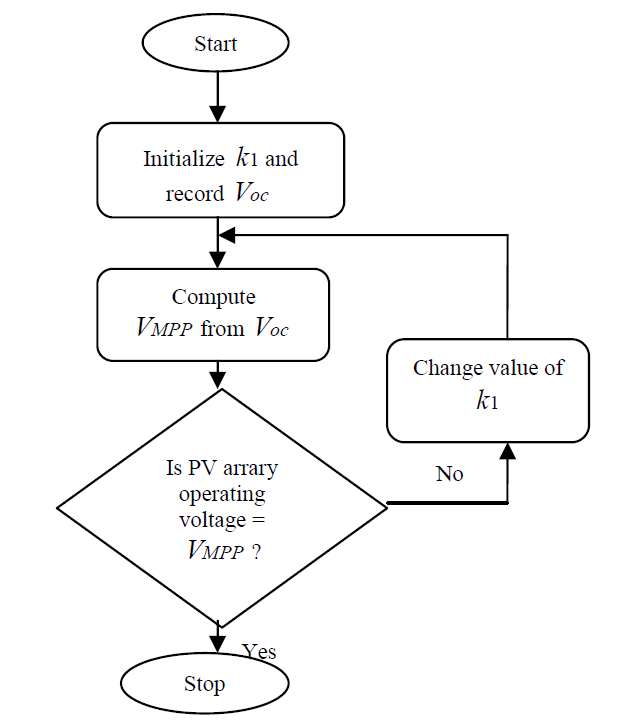
\includegraphics[width=0.4\textwidth]{../Pictures/P1/Flow_chart/Flow_chart_constant_voltage}
		\caption{flow chart constant voltage\cite{flowchartVC}. }
		\label{fcconstantvoltage}
	\end{center}	
\end{figure}

\subsection{Perturb and observe}
With the method "perturb and observe", the currently measured power is periodically compared with the previous power. If the measured power is greater than the power from the previous measurement, the algorithm is moving in the right direction to the MPP. If a power reduction is detected after the comparison, the algorithm is moving away from the MPP. The next step is the identification of a voltage increase or reduction to regulate the voltage for getting the MPP voltage. This depends on which side of the MPP the algorithm is working. If the algorithm detects less voltage than the MPP, the voltage for the next step should increase. If more voltage than the MPP is detected,the algorithm decreases the voltage for the next step to reach the MPP.
The flowchart in the figure \ref{fcperturbandobserve} illustrates this method. The classical algorithm uses a fixed step to change the voltage. When the MPP is reached, the algorithm oscillates around the MPP\cite{flowchartVC}. 

The required computing power of the perturb and observe algorithm is also low, because it is easy to compute. The algorithm contains the calculation of the power and the comparison with previous power for each step. Another advantage of perturb and observe is that a current sensor does not necessarily have to be used. There are scientific paper where only a voltage sensor is used \cite{withoutcurrent}.There is a disadvantage when the algorithm is near to the MPP since, at this point, the algorithm oscillates around the MPP, so that the MPP cannot be reached exactly. The oscillation depends on the value of the fixed step. If the fixed step value is high, the MPP will be reached quickly. On the other hand, the oscillation around the MPP is high, which reduces the efficiency. The advantage of a small value is that the oscillation is small, but it takes more time to reach the MPP\cite{AN1521_MC}. 

\begin{figure}[htbp]
	\begin{center}
		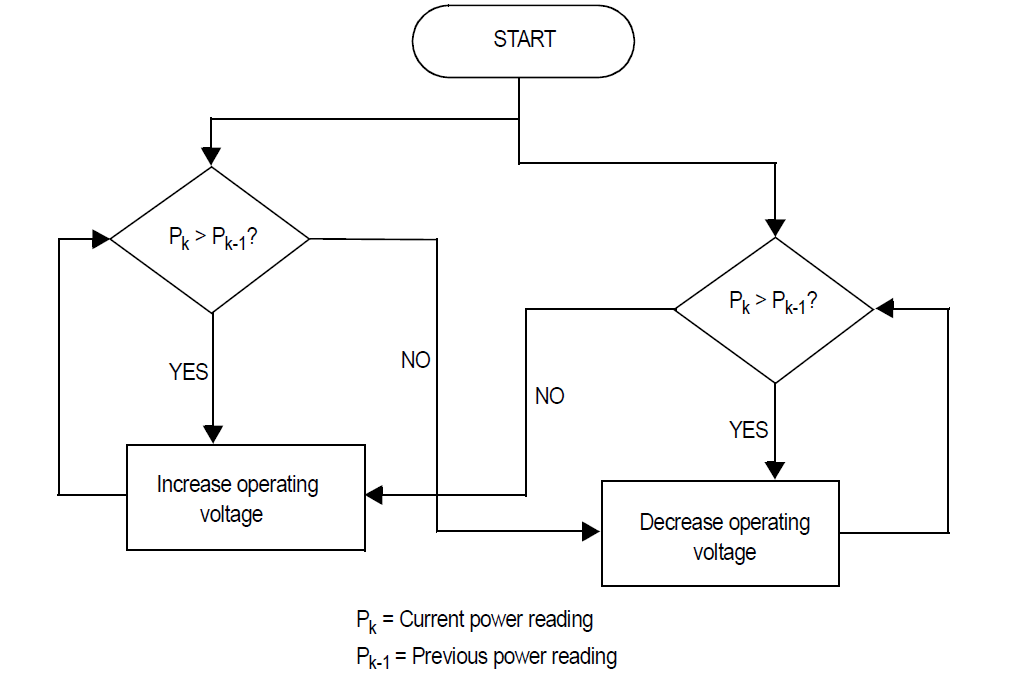
\includegraphics[width=0.8\textwidth]{../Pictures/P1/Flow_chart/flow_chart_perturb_observe}
		\caption{flow chart from perturb and observe\cite{PerturbObserveFC}.}
		\label{fcperturbandobserve}
	\end{center}	
\end{figure}

\subsection{Incremental conductancee}
The approach of incremental conductance is that the MPP is at the position where the derivative of the power with respect to the voltage is 0. On the left side of the MPP the derivative is greater than 0 while on the right side it is less than 0, this behavior is described by the following equations.
\begin{equation} \label{Inccond1}
\frac{dP}{dV} = 0 ,\; at\; MPP 
\end{equation} 
\begin{equation} \label{Inccond2}
\frac{dP}{dV} > 0 ,\; left\; side\; from\; MPP 
\end{equation}
\begin{equation} \label{Inccond3}
\frac{dP}{dV} < 0 ,\; right\; side\; from\; MPP
\end{equation}
The algorithm compares the incremental conductance with the previous one to increase (left side of MPP) or decrease (right side of MPP) the voltage. After the MPP has been reached, the algorithm is stopped. Thus, there will be no oscillation around the MPP. If a change in the current is detected, the algorithm starts to find the MPP again, as you can see in the flowchart in the figure \ref{fcinccon}\cite{AN1521_MC}.

An advantage of incremental conductance is remaining exactly at the MPP that when this is reached. This increases the efficiency of the PV panel. As with perturb and observe, a fixed value is used to change the voltage. If the value is high, the probability is higher that the algorithm oscillated around the MPP. 
Two sensors are used for the implementation. In addition, the microcontroller requires a higher computing power than perturb and observe, since many more commands are called up during an iteration step. The costs for the algorithm development and microcontroller are higher compared to the other two algorithms\cite{AN1521_MC}.
\begin{figure}[H]
	\begin{center}
		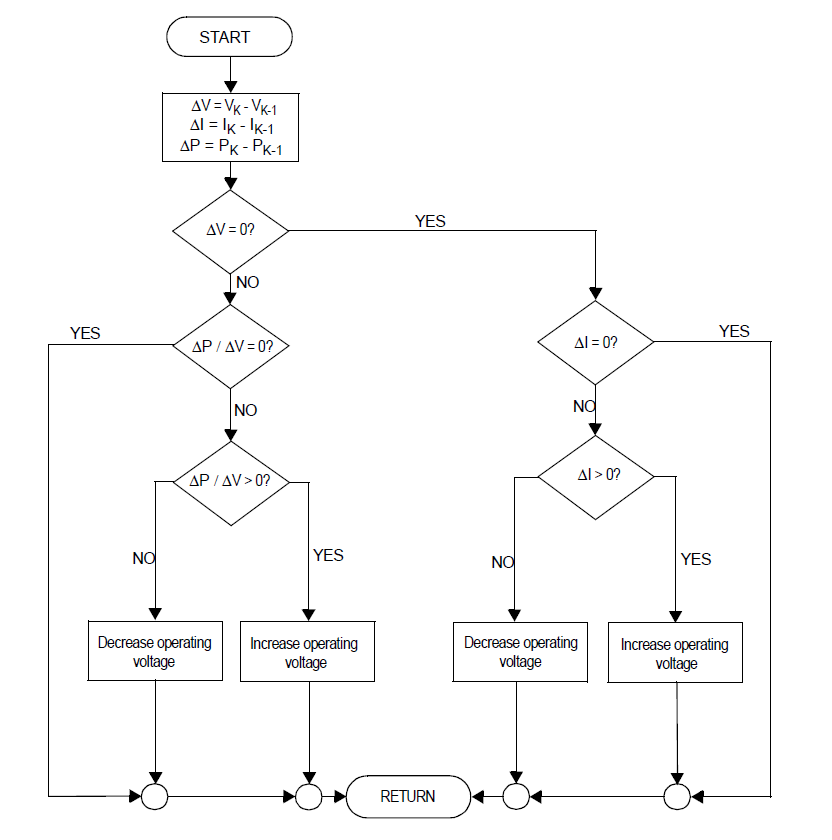
\includegraphics[width=0.63\textwidth]{../Pictures/P1/Flow_chart/flow_chart_incremental_conductance}
		\caption{flow chart incremental conductance \cite{AN1521_MC} }
		\label{fcinccon}
	\end{center}	
\end{figure}

%Table \ref{summaryMPPT} gives an overview of the advantages and disadvantages of the different algorithms.
%%\begin{table}[H] 	
%	\centering 
%	\begin{tabular}  {|>{\centering}m{2cm}|>{\centering}m{2cm}|>{\centering}m{2cm}|>{\centering}m{2cm}|>{\centering}m{2cm}|>{\centering}m{2cm}|}
%		\hline
%		\rowcolor{lightgray}						 \textbf{MPPT Algorithm} & 	
%		\textbf{Sensed Parameters} &
%		\textbf{Micro-controller Computation} &
%		\textbf{Complexity}&
%		\textbf{Reliability}	&
%		\textbf{Overall Cost}
%		\tabularnewline  \hline
%		Constant voltage 	& Voltage 		& Absent/Low &  Very simple & Not accurate & Low 										\tabularnewline \hline
%		Perturb and observe & Voltage + Current  & Low  &  Medium & Not so much accurate & Low/ Medium 		\tabularnewline \hline
%		Incremental conductance & Voltage + Current & Medium &  Medium/ High & Accurate and operate at MPP & Low/ Medium	\tabularnewline	\hline
%	\end{tabular} \label{tab:summaryMPPT}
%	\caption{Summary  of the MPPT algorithm \cite{flowchartVC} }
%
%\end{table}



